\section{Wstęp}
%Część ta~zawiera wstępne informacje o~realizowanym projekcie. Zebrano w~nim wszystko to~co było dostępne zanim student przystąpił do~realizacji informatycznej części projektu. Opisano stanowisko laboratoryjne na~którym powstał projekt.

\subsection{Geneza}
Tematem projektu, którego dotyczy to~sprawozdanie jest: Gas Analyzer". Pomysł na~projekt pojawił~się w~wyniku nawiązania przez nas współpracy z~Zakładem Kotłów i~Wytwornic Pary, a~dokładnie Panem Tomaszem Kress.

\subsection{Temat}
Głównymi celami pracy było napisanie oprogramowania umożliwiającego gromadzenie danych pomiarowych z~kilku urządzeń firmy Siemens.

\subsection{Stanowisko}
W~czasie realizacji projektu wykorzystywaliśmy 2~różne stanowiska. W~pierwszej fazie projektu korzystaliśmy z~uproszczonego stanowiska, które wyglądało jak na~Rysunku~\ref{schemat1}. W~dalszej fazie projektu, kiedy mieliśmy już przygotowaną i~przetestowaną wersję podstawową współpracującą z~jednym urządzeniem pomiarowym rozpoczęliśmy pracę na stanowisku docelowym składającym się z~4 urządzeń, które wyglądało jak na Rysunku~\ref{schemat2}.
\subsubsection{Stanowisko prototypowe}
\begin{figure}[!htb] 	\centering 	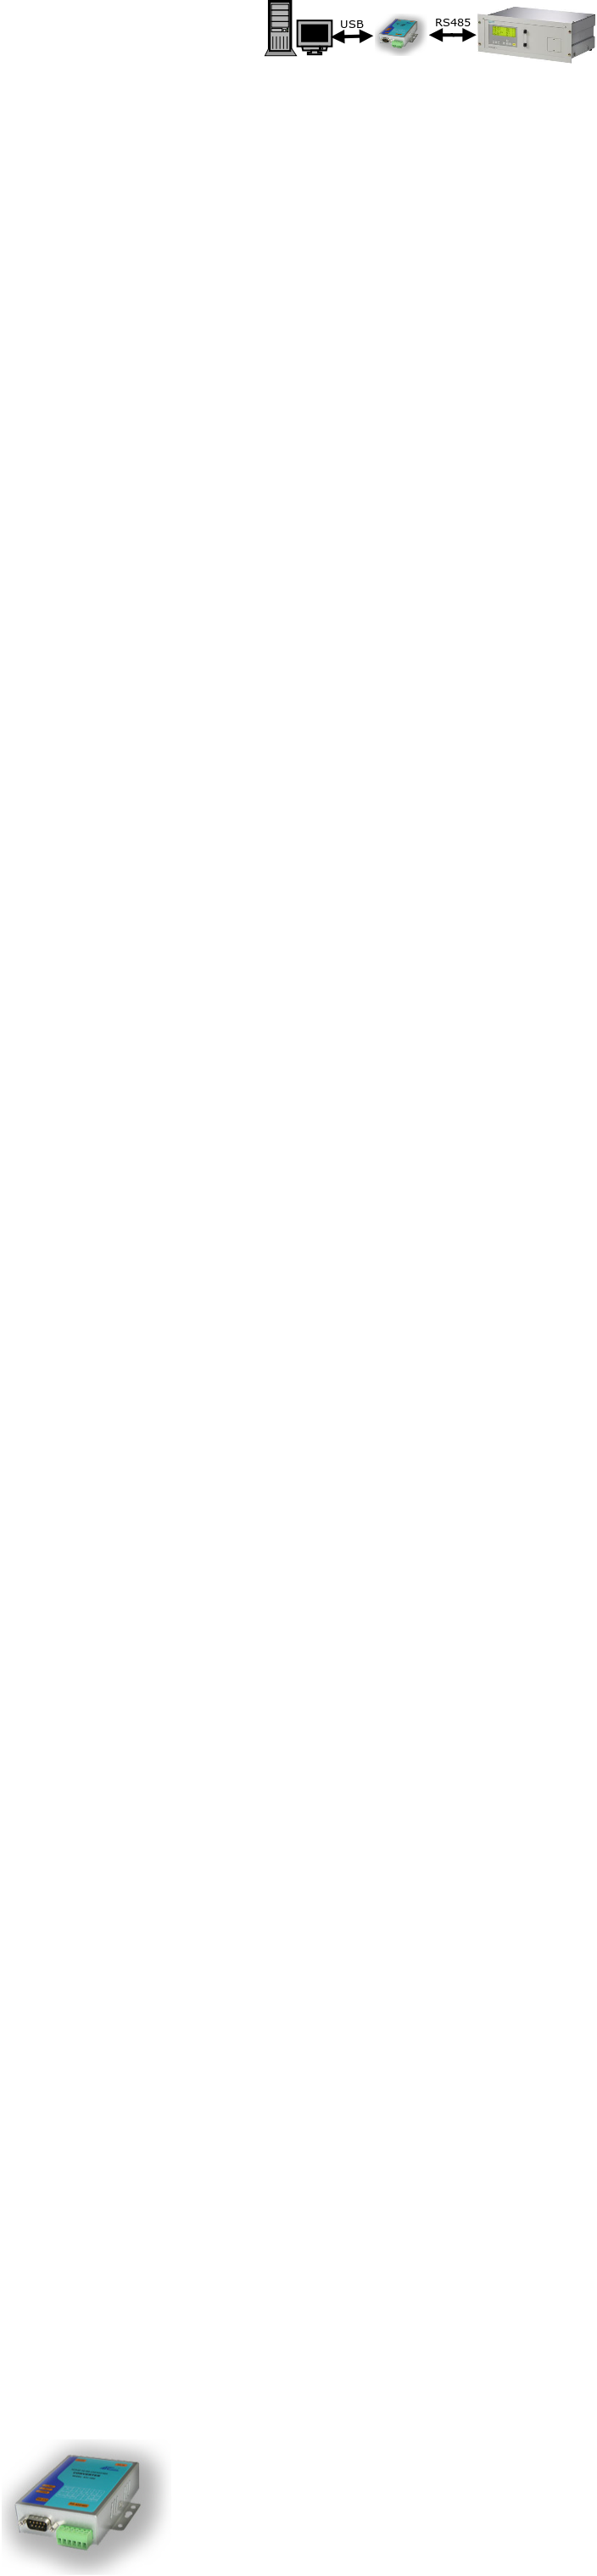
\includegraphics[width=0.8\textwidth]{images/schemat1} 	\caption{Schemat stanowiska prototypowego} \label{schemat1} \end{figure} 
Na~potrzeby realizacji projektu stworzono stanowisko laboratoryjne, którego schemat przedstawia Rysunek~\ref{schemat1}. Składa się ono~z:
\begin{itemize}
\item Komputera,
\item Konwertera ATC-850,
\item ULTRAMAT 23.
\end{itemize}
\indent
\indent Komputery na, których powstała wersja rozwojowa projekty pracowały na systemach operacyjnych Linux Ubuntu w~wersji 32 oraz 64~bitowej. Do~połączenia komputera z~urządzeniem ULTRAMAT~23 zastosowano izolowany konwerter~USB do~RS-232/422/485, moduł ATC-850 jest automatycznie wykrywany i~instalowany jako standardowy port~COM. Stosowane w~tej fazie projektu urządzenie pomiarowe potrafiło mierzyć zawartość $ CO $, $ CO_2 $, $ NO $ oraz $ O_2 $.

\subsubsection{Stanowisko docelowe}
\begin{figure}[!htb] 	\centering 	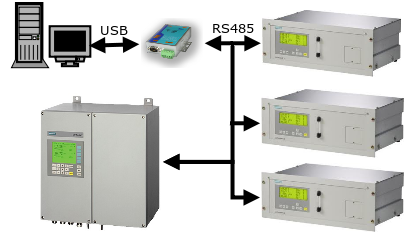
\includegraphics[width=0.7\textwidth]{images/schemat2} 	\caption{Schemat stanowiska docelowego} \label{schemat2} \end{figure} 
Docelowo zrealizowany projekt ma być uruchamiany na~stanowisku, którego schemat przedstawia Rysunek~\ref{schemat2}. Składa się ono~z:
\begin{itemize}
\item Komputera,
\item Konwertera ATC-850,
\item 3x ULTRAMAT 23,
\item ULTRAMAT 6.
\end{itemize}
\indent
\indent Stanowisko docelowe różni się od stanowiska prototypowego po pierwsze systemem operacyjnym, który pracuje na komputerze i jest to Windows XP. Po drugie stanowisko docelowe posiada więcej urządzeń pomiarowych, a jest ich dokładnie cztery i mierzą wartości przedstawione w Tabeli~\ref{tab:docelowe}.

\begin{table}[h]
\centering
\begin{tabular}{|l|l|}
\hline Urządzenie & Wielkości mierzone \\ 
\hline ULTRAMAT~6 & $ NH_3 [vpm] $ \\ 
\hline ULTRAMAT~23 & $ CH_4 [\%], CO [\%], CO_2 [\%], O_2 [\%] $ \\ 
\hline ULTRAMAT~23 & $ CO [ppm], CO_2 [\%], NO [ppm], O_2 [\%] $ \\ 
\hline ULTRAMAT~23 & $ CO [ppm], SO_2 [ppm], NO [ppm], O_2 [\%] $ \\ 
\hline 
\end{tabular} 
\caption{Urządzenia docelowe wraz z wartościami mierzonymi}
\label{tab:docelowe}
\end{table}

\subsection{Analiza tematu}
Analiza tematu polegała przede wszystkim na zapoznaniu się z~dokumentacjami urządzeń \cite{u23,u6}. Szczególnie istotnym, a w~zasadzie najważniejszym punktem całej analizy były interfejsy i~protokoły dostępne w obu typach urządzeń oraz w ewentualnych kolejnych urządzeniach tego producenta. \\ \newline
Analiza pozwoliła wytypować do dalszej analizy dwa protokoły:
\begin{enumerate}
\item PROFIBUS-DP/-PA
\item ELAN Network
\end{enumerate}
Szczegółowa analiza rozwiązań opartych o oba protokoły komunikacyjne w dokumentacjach producenta \cite{elan,step7,comm} pozwoliła ustalić, że w~przypadku PROFIBUSA można zastosować sterownik przemysłowy wyposażony w odpowiednie złącze komunikacyjne lub rozszerzony o~odpowiedni moduł. Niestety jest to rozwiązanie drogie i~mało elastyczne. Teoretycznie funkcjonują na rynku przejściówki PROFIBUS~$ \Leftrightarrow $~USB, ale nie~udało nam~się znaleźć niczego aktualnego i~godnego rozważań. Najistotniejszym punktem analizy był protokół ELAN Network, dostępna do~niego dokumentacja \cite{elan} uświadomiła nam, że spełnia wszystkie nasze wymagania, a sprzęt potrzebny do uruchomienia jest tani i~ogólnodostępny. Własna implementacja tego protokołu na podstawie dokumentacji i~testów pozwala na~pełną elastyczność i dopasowanie do naszych potrzeb.
Poznanie tych podstaw pozwoliło dobrać technologię odpowiednią do~realizacji projektu zgodnie z~założeniami. Ostatecznie wybór padł na ELAN Network oraz stworzenie własnego oprogramowania w Javie.

\subsection{Założenia}
Oprogramowanie do zbierania danych pomiarowych powinno zostać stworzone przy użyciu technologii pozwalającej działać na~różnych systemach operacyjnych bez~skomplikowanych zabiegów. Funkcjonalności wchodzące w~skład projektu,~to:
\begin{itemize}
\item wykorzystanie jednego z dostępnych w urządzeniach protokołów,
\item automatyczne wykrywanie podłączonych urządzeń,
\item zarządzanie użytkownikami, tytułami naukowymi, miejscami, obiektami itd.
\item wizualizacja bieżących pomiarów,
\item wykrywanie i sygnalizacja problemów z urządzeniem,
\item zapisywanie bieżących pomiarów ze wszystkich urządzeń jednocześnie,
\item regulowany krok zapisu pomiarów do~bazy,
\item możliwość dodania komentarza do~zapisywanego pomiaru,
\item generowanie raportu z~pomiaru jako plik arkusza kalkulacyjnego,
\item generowanie raportu z~pomiaru jako plik do wydruku z~wynikami np. format~PDF,
\item konfiguracja nazwa urządzeń widocznych w aplikacji,
\item ustawianie precyzji pomiarów dla danej wielkości mierzonej.
\end{itemize}
\indent
\indent Powyżej zostały wymienione założenia podstawowe, jednak autorzy nie~wykluczają zrealizowania dodatkowych zadań, które nie~zostały zamieszczone w~pierwotnej koncepcji realizacji projektu.

\subsection{Plan pracy}
Realizacja projektu została podzielona na następujące etapy:
\begin{itemize}
\item Przygotowanie stanowiska, zebranie odpowiednich materiałów i~literatury,
\item Analiza wymagań funkcjonalnych aplikacji,
\item Projektowanie struktury oprogramowania i~interfejsów wymiany danych,
\item Implementacja,
\item Testowanie i~uruchamianie,
\item Przedstawienie projektu i~ewentualne korekty.
\end{itemize}
\indent
\indent Powyższy plan pracy stanowił dla autorów wyznacznik kolejnych działań. Jednak powszechnie wiadomo, że w~praktyce poszczególne punkty są~wymienne i~wpływają na siebie wzajemnie. Dodatkowo na potrzeby realizacji projektu powstał szczegółowy plan wraz z~terminami oraz osobami odpowiedzialnymi za poszczególne zadania przedstawiony w~Tabeli~\ref{tab:harmonogram}

\begin{table}[h]
\centering
\begin{tabular}{|p{0.15\textwidth}|p{0.1\textwidth}|p{0.75\textwidth}|}
\hline \textbf{Termin} & \textbf{Osoba} & \textbf{Zadanie} \\ 
\hline\hline 11.03 -- 17.03 & Wszyscy & Wybór tematu. \\ 
\hline 18.03 -- 20.03 & Wszyscy & Określenie celu i~zakresu, przygotowanie harmonogramu, podział zadań. \\ 
\hline 21.03 & Wszyscy & Analiza sprzętu oraz dokumentacji. \\ 
\hline 22.03 -- 23.03 & Wszyscy & Analiza oraz porównanie dopuszczalnych rozwiązań z wykorzystaniem protokołu ELAN lub~Profibus. \\ 
\hline 24.03 -- 25.03 & Wszyscy & Analiza wybranego protokołu oraz potrzebnego sprzętu do połączenia z komputerem (np. konwerter RS-485 $\Leftrightarrow\Leftrightarrow$ USB ). \\ 
\hline 25.03 -- 02.04 & Wszyscy & Implementacja wybranych fragmentów protokołu. \\ 
\hline 29.03 -- 17.04 & Damian & Przygotowanie podstawowej wersji interfejsu użytkownika, umożliwiającej przetestowanie implementacji protokołu. \\ 
\hline 03.04 -- 18.04 & Grzegorz & Rozwinięcie podstawowej wersji protokołu – interpretacja i~przetwarzanie odbieranych danych. \\ 
\hline 20.04 -- 01.05 & Grzegorz & Stworzenie modelu bazy danych i~połączenia ORM. \\ 
\hline 19.04 -- 05.05 & Damian & Wykrycie i wizualizacja struktury sieci oraz odbieranych danych. \\ 
\hline 03.05 -- 06.05 & Damian & Generowanie PDF. \\ 
\hline 04.05 -- 10.05 & Grzegorz  & Generowanie XLS. \\ 
\hline 13.05 -- 22.05 & Grzegorz & Zarządzanie ustawieniami urządzeń. \\ 
\hline 27.05 -- 05.06 & Damian & Poprawki w GUI. \\ 
\hline 01.06 -- 08.06 & Wszyscy & Instrukcja użytkownika oraz dokumentacja. \\ 
\hline 
\end{tabular} 
\caption{Szczegółowy plan pracy wraz z~harmonogramem i~osobami odpowiedzialnymi}
\label{tab:harmonogram}
\end{table}
